\section{Conformal Invariance and Criticality}
\label{ch-conf}

Lorem ipsum dolor sit amet, consectetur adipisicing elit, sed do eiusmod tempor
incididunt ut labore et dolore magna aliqua. Ut enim ad minim veniam, quis
nostrud exercitation ullamco laboris nisi ut aliquip ex ea commodo consequat.
Duis aute irure dolor in reprehenderit in voluptate velit esse cillum dolore eu
fugiat nulla pariatur. Excepteur sint occaecat cupidatat non proident, sunt in
culpa qui officia deserunt mollit anim id est laborum.

\begin{figure}
\begin{center}
    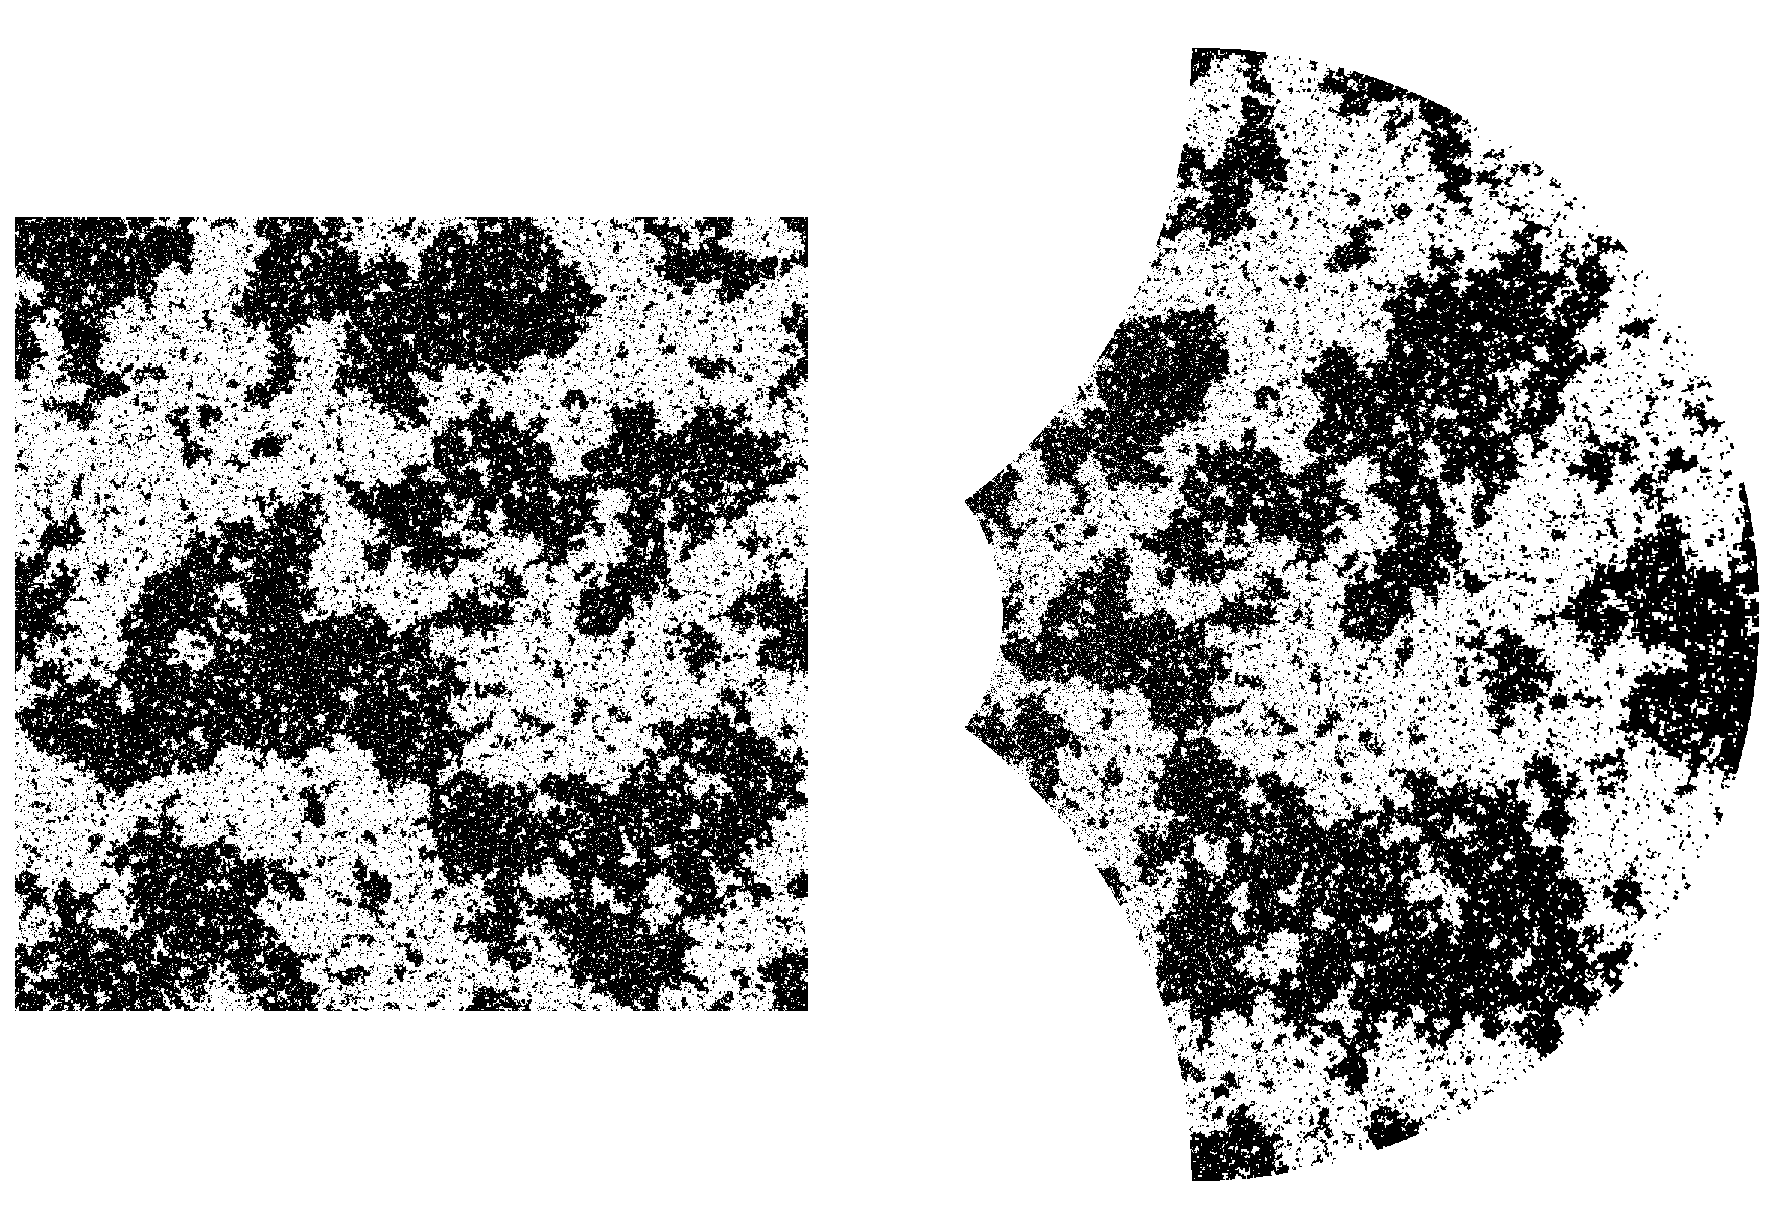
\includegraphics[scale=0.5]{chapters/ch3-conf/figs/isingcm}
\end{center}
\caption{Critical Ising model simulated on a $1024\times1024$ square lattice
    with the clusters colored according to their size. When subject to a
    conformal transformation $f(z)=\exp{\left(2z+1/2+i\pi/2\right)}$, the image
    gets distorted, although the overall structure of the clusters (which
    implies the structure of correlations) is preserved.}
\label{fig:isingcm}
\end{figure}


%\begin{figure}
%\begin{center}
    %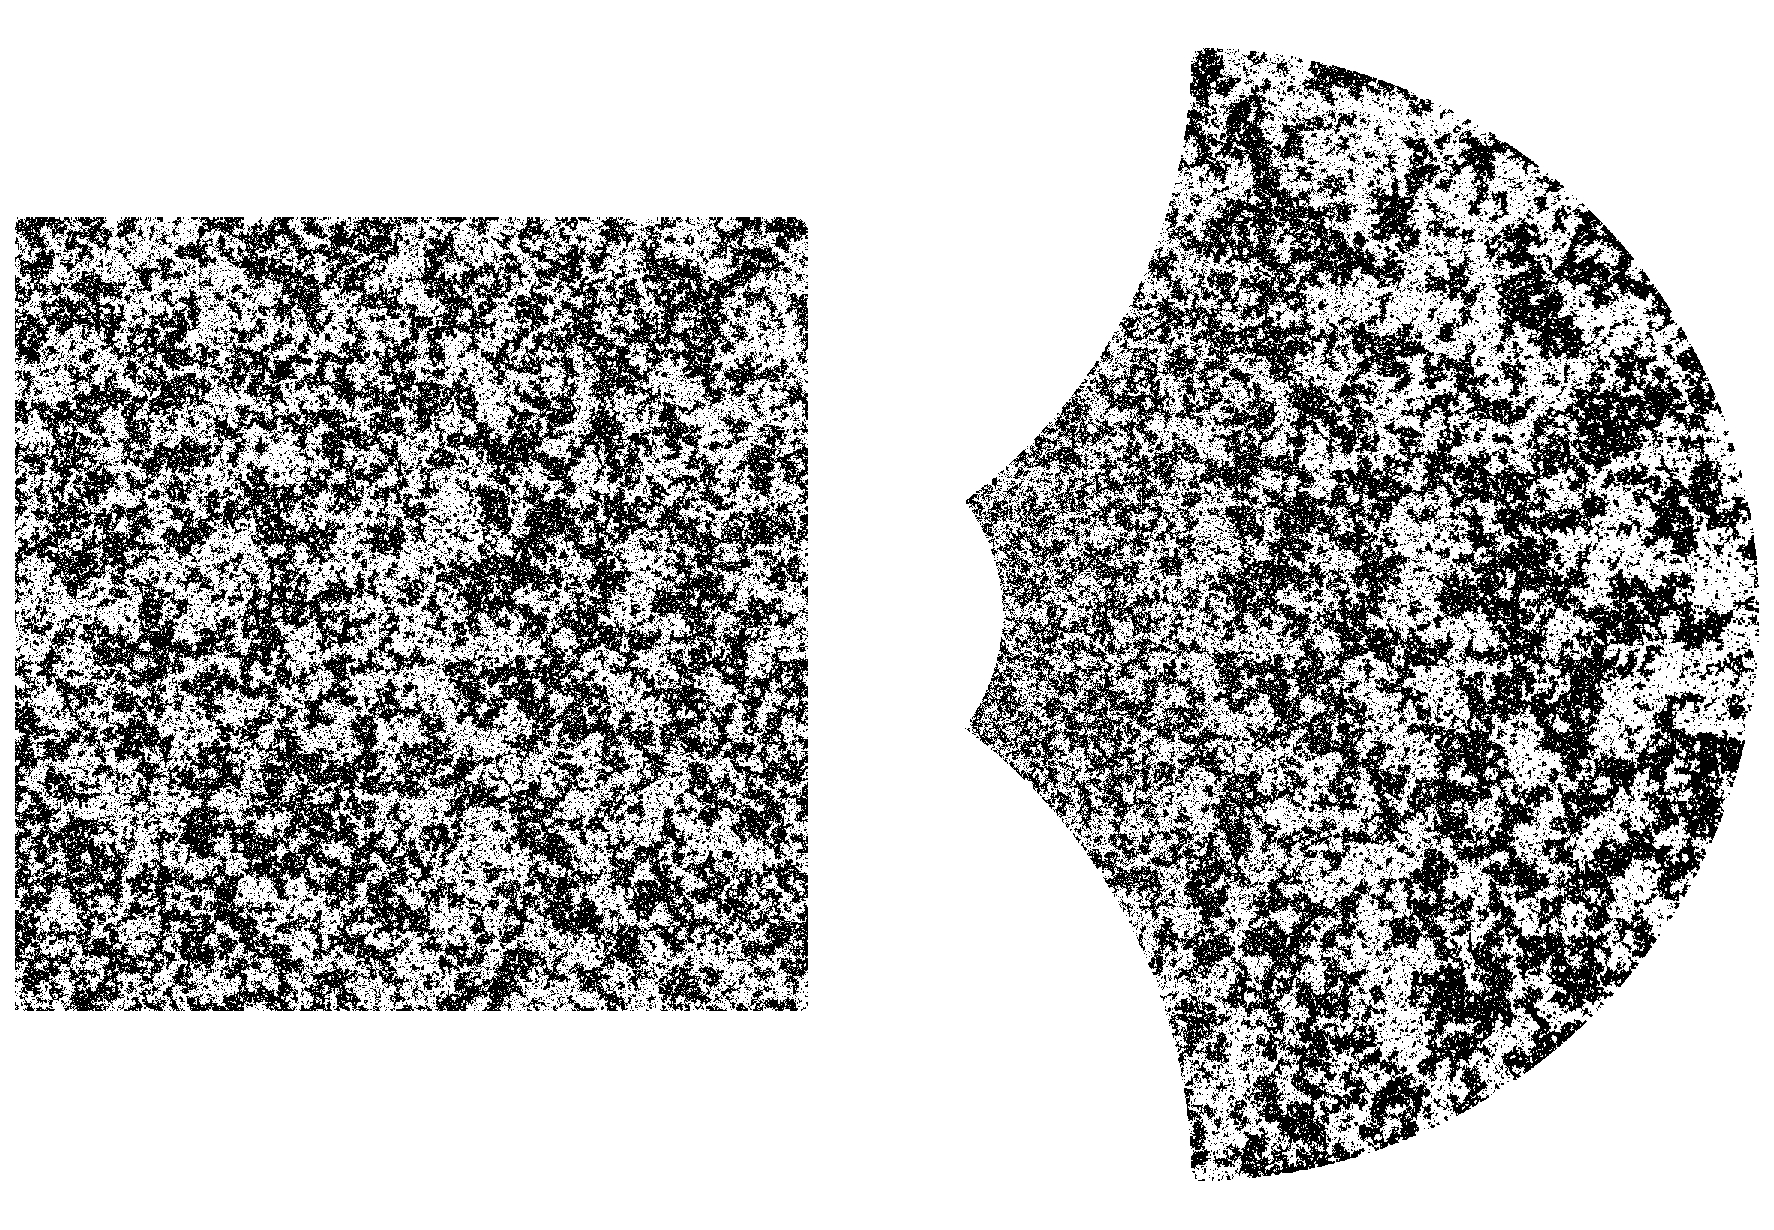
\includegraphics[scale=0.5]{chapters/ch3-conf/figs/isingcm2}
%\end{center}
%\caption{Ising model above the critical point simulated on a $1024\times1024$
    %square lattice. When subject to the conformal transformation
    %$f(z)=\exp{\left(2z+1/2+i\pi/2\right)}$, the get ``squished'' or stretched
    %altering the distribution of clusters.}
%\label{fig:isingcm2}
%\end{figure}
